\documentclass{article}
\usepackage[utf8]{inputenc} % allow utf-8 input
\usepackage[T1]{fontenc}    % use 8-bit T1 fonts
\usepackage{hyperref}       % hyperlinks
\usepackage{url}            % simple URL typesetting
\usepackage{booktabs}       % professional-quality tables
\usepackage{amsfonts}       % blackboard math symbols
\usepackage{nicefrac}       % compact symbols for 1/2, etc.
\usepackage{microtype}      % microtypography
\usepackage{xcolor}         % colors
\usepackage[final, nonatbib]{neurips_2022}
\usepackage{float}
\usepackage{subcaption}
\usepackage{comment}
\usepackage{amsmath, amssymb}
\usepackage{bbm}
\usepackage{stackengine}
\usepackage{minted}
\usepackage{cite}
\usepackage{import}
\usepackage{xifthen}
\pdfminorversion=7
\usepackage{pdfpages}
\usepackage{transparent}

\usepackage{listings} % User package for writing Code in the Appendix
\RequirePackage{lineno}
\linenumbers

\lstset{ % Set the default style for code listings
	numbers=left,
	numberstyle=\scriptsize,
	numbersep=8pt,
	basicstyle=\scriptsize\ttfamily,
	keywordstyle=\color{blue},
	stringstyle=\color{red},
	commentstyle=\color{green!70!black},
	breaklines=true,
	frame=single,
	language=bash,
	tabsize=4,
	showstringspaces=false
}


\makeatletter
\renewcommand{\@noticestring}{}
\makeatother
\title{Do (wo)men talk too much in films?}
\begin{document}
\author{Authors: Jannes van Poppelen, Linus Falk, Steven Bijl, Niklas Kostrzewa}
\maketitle

\begin{abstract}
    In this work, we train different machine learning models using a data set of 2000 Hollywood movies in order to accurately predict the sex of the lead role of a movie, given a list of features corresponding to each movie. Even though the training data is heavily biased towards a male lead, all trained models end up outperforming a naive classifier that merely predicts a male lead. The generative QDA model was found to give the best performance after a 10-fold cross-validation, as out of all models it has the best mean prediction accuracy of 90\% and a near-vanishing variance. Since the selected input features for this model were only briefly touched, a more thorough optimization for the input features could possibly yield an even more accurate model.
\end{abstract}

\section{Introduction}
A study of 2000 movies has recently shown that white men tend to dominate movie roles \cite{dataset}. Attempting to confirm or deny this finding, multiple machine learning models will be trained using a relatively small data set of Hollywood movies, with the goal to predict the gender of the main actor in Hollywood screenplays. An additional focus will be put on analyzing gender bias for the lead- and co-lead actors. The provided data set has a wide variety of Hollywood movies, ranging over multiple decades and genres. Each entry consists of a total of 14 attributes. The 13 input parameters are the number of actors per gender, gross profit, the total number of words spoken, the number of words spoken per gender, the number of words spoken by lead, the difference in the number of words by lead and co-lead, lead- and co-lead age, and the mean age of male and female characters. The last data entry is the gender of the lead actor, which is the output that should be predicted.

\section{Data Analysis}
In order to get a better understanding of the gender bias within the data we can ask ourselves \emph{which sex dominates speaking roles in Hollywood movies}.
%The first step in machine learning is to take a closer look on the provided data to get an better understanding of it and clean it from outliers and empty entries if needed. In order to get familiar with the data it is helpful to ask some related question about the data.Since we want a model that can predict the gender of the lead character we ask questions related to this. A good start would be to investigate \emph{if men or women dominate speaking roles in Hollywood movies?} 
By summing and comparing the number of male- and female actors for all movies in the data set we can clearly see that there is male dominance in speaking roles, as is shown in figure \ref{fig:dataanalysis}. While this is a nice static observation, it makes more sense to ask the question in a dynamic context, by studying how this dominance has changed over time.
%How this changed over time is a relevant question also, so we ask: \emph{has gender balance in speaking roles changed over time (i.e. years)?}. 
To do this we start by calculating the percentage of female actors in each film year by year. Then, using NumPy's polyfit function, a straight line is fitted to the data. The resulting line shows a  positive trend, indicating that the percentage of female actors per movie is increasing, but is still not close to 50 \%. Next, we can examine economic differences between male- and female-dominated movies, where the most straightforward would be to analyze \emph{if male-dominated movies generate more gross than female-dominated movies.}
%Next step would be to examine if there is any economic differences between movies with more male speaking or in other words: \emph{Do films in which men do more speaking make a lot more money than films in which women speak more?}. 
By sorting out all movies by the gender with the most words spoken and calculating the mean gross we can see that indeed male-dominated movies generate more gross, which is seen in the lower plot in figure \ref{fig:dataanalysis}. 
%movies with more male speaking generate more 'Gross' then movies with more female speaking, see figure: \ref{fig:dataanalysis}. 
In order to get a bigger look at the data set and locate outliers, a histogram and pairwise scatter plot of the normalized features are made. These can also indicate obvious correlations between the features. The plot is found in the appendix in figure \ref{fig:scatter}, which does confirm the existence of some outliers. Since all features are numerical, there is no need for 'dummy' variables. Most features do not follow a normal distribution, which makes it difficult to exclude the outliers without transforming the data. Another way to analyze the data would be to compute the covariance matrix, by calculating the covariance between all features $\text{cov}(X,Y) = \frac{1} {n} \sum_{i=1}^{n} (x_i-E(X))(y_i-E(Y))$ \cite{smlbook}, however, since the majority of the features does not follow a normal distribution, this would again be of limited use.

%The next step in the data analysis is to examine the data set and locate outliers by making a histogram and pairwise scatter plot of the normalized features \cite{scatter_mat}. Doing this allow us to see how the data is distributed and also if there are any obvious correlations between the features. Examining the histogram scatter plot, figure \ref{fig:scatter} in the appendix indicate that there are several outliers in the data set. We can also conclude that all features are numerical there is no need for 'dummy' variables for classification features. Since most of the features don't have a normal distribution it would be difficult to exclude these extreme values with a statistical method without transforming the data first. Another method to examine the data set is to make a covariance matrix by calculating the covariance between the features: $\text{cov}(X,Y) = \frac{1} {n} \sum_{i=1}^{n} (x_i-E(X))(y_i-E(Y))$ \cite{smlbook}. The expected value is used and since the majority of the features data is not normally distributed it would be of limited use. 

\begin{figure}[ht!]
    \centering
    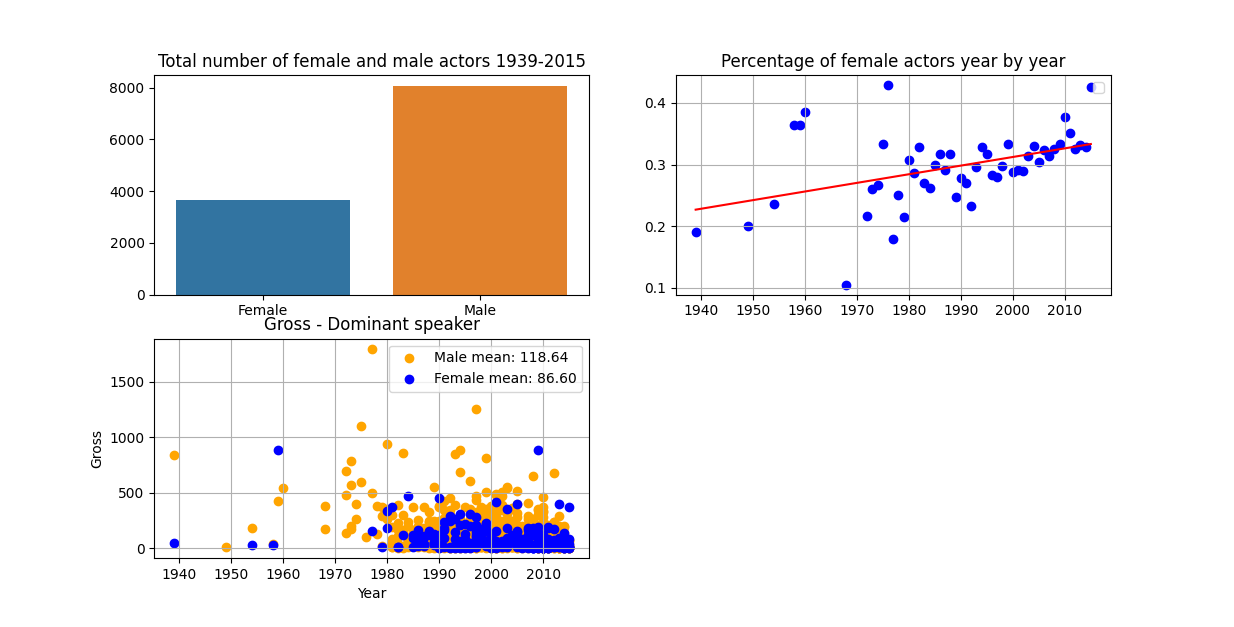
\includegraphics[width=120mm]{img/data_analysis.png}
    \caption{Various plots analyzing the gender bias in Hollywood movies.}
    \label{fig:dataanalysis}
\end{figure}

\section{Implementation of methods}
There is an abundance of machine learning methods used for classification problems. This analysis, however, restricts itself to 5 different methods, these being logistic regression, discriminant analysis, $k$-nearest neighbour model, tree-based methods, and deep learning. The analysis of most of these methods relies heavily on the concept of cross-validation. This is a statistical technique used to test and train these models, by splitting the data set into training- and validation sets, whence the final error is obtained upon averaging the previously obtained errors.

\subsection{Logistic regression}
Logistic regression is a classification model, while the name itself could suggest something else. Here we present a short description of the fundamentals behind the model, and how to implement and tune it for this specific problem. Assuming the reader has a basic understanding of linear regression we can start from there and build our logistic regression model: $z = \theta_0 + \theta_1x_1 + \theta_2x_2 + \ldots + \theta_px_p$. To fit our model to a prediction of probability $\text{p}(y = 1 | x) $ we use the logistic function also known as the Sigmoid function, which is defined as $f(\text{z}) = \frac{e^{z}} {1 + e^{z}} \in \begin{bmatrix} 0& 1 \end{bmatrix}$. Given the probability of one class in the case of a classification problem with 2 classes, we have the probability for the second class $\text{p}(y = -1 | x)$= $ 1 - f(\text{z})$. By choosing 1 and -1 as the labels we can simplify our expressions such that we are left with $f(\text{z}) = \frac{e^{z}} {1 + e^{z}} = 1 - f(\text{z}) = \frac{e^{\theta^{T}x}} {1+e^{\theta^{T}x}}$. Next, by using the training data, the goal is to find an optimal set of parameters $\hat{\theta}$ for the model. Using the maximum likelihood approach we find $\hat{\theta} = \text{arg max p(\textbf{y} $|$ \textbf{X;$\theta$})} = \text{arg max} \sum_{i=1}^{n} \text{ln } \text{p(y}_i | \textbf{x}_i;\theta)$, which can be turned into a minimization problem by using the negative log-likelihood as the cost function. Since the labels are chosen in a clever way, we end up with the cost function: $J(\theta) = \frac{1} {n} \sum_{i=1}^{n} \text{ln}(1+e^{-y_i\theta^{T}x_i})$. Then, the optimal parameters for the logistic regression model is found by solving the minimization problem
\begin{equation}
\hat{\theta} = \text{arg min} \frac{1} {n} \sum_{i=1}^{n} \text{ln}(1+e^{-y_i\theta^{T}x_i})
\end{equation}

However, this modification to the regression model is not "perfect", as there exists no closed-form solution. To find the parameters $\hat{\theta}$, the minimization problem has to be solved numerically \cite{smlbook}. In the scikit-learn library, different numerical solvers for the logistic regression model can be chosen, all of which have their own pros and cons. This hyperparameter is one that can be tuned in logistic regression. Others are the type of regularization and its strength.\\

\noindent Regularization is a method to decrease the flexibility, or in other words, to avoid overfitting the training data. To achieve this, a penalty term is added to the loss function. L1 regularization penalizes the parameter weights in proportion to the sum of the absolute value of the weights. This penalty can drive the weight for an irrelevant feature parameter to 0. An other option is L2 regularization, which penalizes the parameter weights in proportion to the sum of squares of the weights. The strength of the penalty is regulated with the coefficient: "Regularization strength" or C in the scikit-learn library. 

Tuning the model further can be done by optimizing the features that are used. Since the features in the data set are all related to the problem and there is no simple way to exclude any of them One option is therefore to test all possible combinations of features by "brute forcing". 

We start tuning the model by testing different solvers using the default settings for the other hyperparameters. First, a model is trained and tested using 10-fold cross-validation, after which the solver and set of features is picked out. Since some of the solvers have convergence problems with non-normalized data, the standardScaler and MinMaxScaler from the scikit-learn library are used to scale the input data. Even though all features are not normally distributed, it proved empirically better to use standardScaler rather than MinMaxScaler. The test resulted in the following solver: 'lbfgs' and set of features: 'Number words female', 'Number of words lead', 'Difference in words lead and co-lead', 'Number of male actors', 'Number of female actors', 'Number words male', 'Mean Age Male', 'Age Lead', 'Age Co-Lead'. 

Next, the remaining optimal set hyperparameters to the logistic regression model, these being the type of regularization and its strength, are found by again testing all possible combinations and seeing which combinations perform best in a 10-fold cross-validation. A useful package from scikit-learn library is GridSearchCV,  which allows us to set up lists of regularization methods and strengths and test all of them, after which it returns the best combination. The input for the grid search is Solver: 'lbfgs', penalty: ['l2'], C: np.logspace(-3,3,7), which returned the results below. 

\begin{itemize}
    \item \textbf{Model: }LogisticRegression(solver='lbfgs', penalty='l2', C=1.0)
    \item \textbf{Mean accuracy: } 87.5\%
\end{itemize}

Comparing the result to a naive classifier that only predicts a male lead, which has an accuracy of around 75\%, we can see an improvement of about 12\%.
%Interesting to note about the resulting model is that non of the features 'Gross' or 'Year' is used even though the data analysis could suggest that these two features are related to the problem. 


\subsection{Discriminant analysis: LDA, QDA}
The Gaussian Mixture Model (GMM) is a generative model which attempts to model $\text{p}(\textbf{x}, y)$, where $\textbf{x}$ is assumed to be numerical- and $y$ a categorical variable. Here, we will look at two GMMs: Linear Discriminant Analysis (LDA) and Quadratic Discriminant Analysis (QDA). These methods are considered when working with fully labeled data. Unlike the \textit{discriminative} models, the GMM describes the joint distribution of both inputs and outputs. $\text{p}(\textbf{x},y)$ states that, given input parameters $\textbf{x}$, one finds a categorical output $y$ with a certain probability. The GMM makes use of the following factorization of the joint probability density function: $\text{p}(\textbf{x},y)=\text{p}(\textbf{x}|y)\text{p}(y)$. Since $y$ is categorical, the categorical distribution can be written as $\text{p}(y=m)=\pi_{m},$ where the number of classifications ranges from 1 to $m$. Additionally, it is assumed that all probabilities follow a Gaussian distribution $\text{p}(\textbf{x})=\mathcal{N}(\textbf{x}|\mu_{y},\Sigma_y)$, where $\mu_{y}$ is the mean vector of the parameter and $\Sigma_{y}$ the covariance matrix. The GMM model can be trained using a supervised and semi-supervised approach. The goal of GMM is to determine the parameters $\theta=\{\mu_m,\Sigma_m,\pi_m\}^{M}_{m=1}$, which can be achieved using the log-likelihood function, $\hat{\theta}=\mathop{\text{arg}\max_{\text{m}} \text{ln}}p(\mathcal{T}|\theta)$, where $\mathcal{T}=\{\textbf{x}_i,y_i\}^{n}_{i=1}$ is the training data. This yields the following solutions: $\hat{\pi}=\frac{n_m}{n}$,$\hat{\mu}_m=\frac{1}{n_m}\sum_{i}\textbf{x}_i$, and $\hat{\Sigma}_m=\frac{1}{n_m}\sum_i(\textbf{x}_i-\hat{\mu}_m)(\textbf{x}_i-\hat{\mu}_m)^T$, where $n_m$ is the total number of data point in class $m$, and $n$ the total number of data points \cite{smlbook}.


The next step is to use the trained model to make predictions $y_*$, i.e., we want to find $p(y|\textbf{x})$. Using Bayes' rule we get
\begin{equation}
    \text{p}(y|\textbf{x})=\frac{\text{p}(\textbf{x},y)}{\text{p}(\textbf{x})}=\frac{\text{p}(\textbf{x},y)}{\sum^{M}_{j=1}\text{p}(\textbf{x},y=j)}
\end{equation}
The final category is selected by using the largest probability, given the input $\mathbf{x_*}$ 
\begin{equation}
    \hat{y}=\mathop{\text{argmax ln}}_{\text{m}}p(y=m|\textbf{x}_*),
\end{equation}
which is known as the decision boundary. The equation above can be extended to the Quadratic Discriminant Analysis (QDA) method by taking the logarithm. Putting this all together, we get the final equation
\begin{equation}
    \hat{y}_*=\mathop\text{argmax}_{\text{m}}\{\ln\hat{\pi}_m+ln\mathcal{N}(\textbf{X}_*|\hat{\mu}_m,\hat{\Sigma}_m)\}
\end{equation}
Taking the logarithm of the Gaussian distribution then gives rise to a quadratic decision boundary.
\subsubsection{Training and evaluating LDA and QDA models}
In order to complete this task, the scikit-learn library for supervised machine learning was used. This is a tool that makes it easy to implement the training and optimization of LDA and QDA methods. This library has functions for LDA and QDA, which creates the models and optimizes hyperparameters depending on the data that is worked with. The main hyperparameter for the LDA methods is the solver. There are three different solvers: "svd" (singular value decomposition), "lsqr" (least squares solution), and "eigen" (eigenvalue decomposition). When choosing lsqr or eigen, there is an additional parameter that can be tuned, which is the shrinkage parameter. The hyperparameter that was tuned for QDA was the regularization parameter, which ranges from 0 to 1. This parameter tries to combat overfitting and collinearity. Here it was found that the standard svd solver gives the highest accuracy for the LDA method, while a regularization paramater of 0.50 was found for the QDA method.

The next step is feature selection. This way optimized by training the models while withholding one feature from the dataset. Essentially, 13 different data sets were constructed, which in turn created 13 different models. This was tested using the svd solver for the LDA method and with regularization parameter of 0 and 0.50 for the QDA method. Using the LDA method, it was found that the highest misclassification accuracy was found when omitting the data from "Mean Age Female". The highest misclassification accuracy found with the LDA method was 13.5\%. For the QDA it was found that the highest misclassification accuracy was obtained when using a regularization parameter of 0.5 and discarding the data from "Year". The highest misclassification accuracy obtained was 10.1\%.

\subsection{k-nearest neighbour}
From a conceptual point of view, the $k$-nearest neighbour ($k$-NN) algorithm is arguably the most straightforward one. The core idea of the algorithm is to predict similar outputs for those inputs that are in close proximity to each other in parameter space. The $k$-NN algorithm belongs to the class of distance-based machine learning methods, and, despite its simplicity, can be applied to both regression and classification problems. In more detail, suppose we have a set of training data $\mathcal{T}=\left\{(\mathbf{x}_i,y_i)\right\}_{i=1}^n$ and an input $\mathbf{x_{\star}}$ whose output we want to predict. Then, one starts by finding the $k$ closest data points $\left\{\mathbf{x}_i\right\}_{i=1}^k$ to $\mathbf{x_{\star}}$, which gives rise to the name $k$-NN, by computing the distance $||\mathbf{x_{\star}}-\mathbf{x}_i||$ between them. Note that the metric need not necessarily be induced from the $\ell^2$ norm. In fact, every norm induces a metric, which can be used to compute the distance between the input and data points, whose physical interpretation heavily depends on the type of metric that is used. Norms that are frequently used are the $\ell^1$-, $\ell^2$- and the more general $\ell^p$ norm, whose metrics are more commonly known as the Manhattan-, Euclidean-, and Minkowski distance, respectively. Moreover, the inclusion of different norms to compute the distances extends the regular $k$-NN algorithm to the kernel $k$-NN algorithm, where the similarity of data points can be specified according to the used kernel\cite{yu2002kernel}.
Next, once the $k$-NNs are found, a prediction is made depending on the type of problem (regression/classification). For classification with $y$ classes, the prediction then takes the form of $ y_{\mathbf{\star}}=\max_{y} \sum_{(\mathbf{x}_i,y_i)\in\mathcal{T}} \omega_i \mathbbm{1}_{\left\{y=y_i\right\}},$ where $\omega_i\in[0,1]$ are so-called weights and $\mathbbm{1}$ denotes the indicator function. For unweighted classification, all weights are equal to 1, but in the case where one would like to further decrease the importance of the data points furthest away from $\mathbf{x_{\star}}$, their respective weights can be scaled down.\\

\noindent The $k$-NN algorithm for classification is quite rigid, as it only leaves room for the hyperparameter $k$ to be varied, as well as deciding whether or not to classify using weights. While the latter is merely done by setting a flag to yes or no, the former is a bit more flexible and needs to be properly investigated. Furthermore, it is important to note that the $k$-NN model behaves differently for each $k$ depending on which features are used in the input. This investigation concerns therefore both the input features and $k$, simultaneously. While there exist roughly 8200 possible combinations of input features, here, without loss of generality, we restrict ourselves only to combinations of 10, 11, 12, and 13 input features, where a minimum 10 features is set to avoid underfitting the model.\\

\noindent Pipelines from the Scikit-learn python library are used to determine the best combination of input features and $k$, by doing a $10$-fold cross-validation for all of the aforementioned combinations of features, while simultaneously varying $k$ to include 1 to 50 nearest neighbours. Here, every input is normalized so that scaling does not play a role, which is a known issue for the $k$-NN algorithm. The results for various norms and the inclusion/exclusion of weighted classification are presented in table \ref{tab:knn}. For visual clarity and brevity, the exact input features are omitted.
\begin{table}[ht!]
    \centering
    \begin{tabular}{|l|l|l|l|}
    \hline
    Model & Accuracy &  k \\ \hline
    Unweighted $\ell^2$      &  0.864    & 14   \\
    Weighted $\ell^2$      &    0.883     &  12 \\
    Unweighted $\ell^1$      &   0.883       & 8  \\
    Weighted $\ell^1$      &   0.883       & 11  \\
    Unweighted $\ell^3$      & 0.874         & 8  \\ \hline
    \end{tabular}
    \caption{Cross-validation accuracy, the optimal value of $k$, and optimal number input features for different models.}
    \label{tab:knn}
\end{table}
\noindent Three of the models reach the same maximum accuracy. A bigger data set could have allowed for tiny differences in performance, which allows a single optimal model to be found. However, this is not an option, so the weighted $\ell^2$ model has been selected as the best model due to its larger optimal value of $k$, as this allows for more flexibility than the other models. For this model, the accuracy per $k$ is plotted in figure \ref{fig:k_acc}.  \\

\noindent Evident from the figure is that the number of nearest neighbours reaches its optimum very quickly. Moreover, the accuracy quickly drops due to overfitting, as is indicated by the long "tail" for large values of $k$. Finally, the optimal $k$-NN model for the given data uses the input features 'Number words female', 'Total words', 'Difference in words lead and co-lead', 'Number of male actors', 'Year', 'Number of female actors', 'Number words male', 'Mean Age Male', 'Age Lead', 'Age Co-Lead', together with $k=12$.

\subsection{Tree-based methods: classification trees, random forests, bagging}

The basic idea behind tree methods is to split the input space into regions. The splitting is done according to rules, which essentially turns it into a binary tree. At each internal node, a rule $x_j < s$ with input parameter $x_j$ and threshold $s$ decides which branch will be chosen for the given input $x$. The leaf nodes then decide which class is chosen. Each leaf node corresponds to one region. The deeper the classification tree, the finer the partition \cite{smlbook}. For this project, three methods will be explained and tested. Classification trees are the most basic form. Bagging is an algorithm to improve the variance of the classification tree, and Random Forest uses a random subset of multiple trees to even further decrease the variance of the classification tree.

\textbf{Classification Tree:}
To find the best partition, which means minimizing the training error, a greedy recursive binary splitting is used. It splits regions recursively in two half-spaces until a stopping criterion is met. The class prediction in each region can be expressed by $\text{p}(y=m|x_\star)\approx \sum_{l=1}^{L}\hat{\pi}_{lm}\mathbb{I}\{x_\star\in R_l\}$, with the proportion of data points in region $l$ of class $m$ described by $\hat{\pi}_{lm}=\frac{1}{n_l}\sum_{i:x_i\in R_l}\mathbb{I}\{y_i=m\}$. At each internal node, the input variable and threshold with a minimal error are chosen. Common error measurements are Log Loss, Entropy, and Gini index\cite{smlbook}.

\textbf{Bagging:}
Bootstrap Aggregation or Bagging tries to lower the variance without raising the bias. To get a low bias, a tree has to grow deep, which can result in overfitting, yielding a high variance. Multiple slightly different classification trees are trained with different training sets in order to avoid this. Bootstrapping is a technique to create multiple datasets of size $n$ from one separate dataset of size $n$. To obtain multiple data sets from one training set, one samples $n$ times from the training set and repeat this $B$ times to get $B$ data sets. After that, one can learn $B$ models whereafter averaging over them results in a low variance.

\textbf{Random Forest:}
Since the individual models used in Bagging are correlated, the variance reduction is limited. The Random Forest approach tries to fix this issue by using only a random subset of inputs as splitting variables at each internal node. This results in more different individual trees since dominant input variables are not picked all the time. Computationally this is also better, as it allows for calculations to be done in parallel, on top of using smaller subsets of variables. %This also results in computational gains, like the ability to calculate parallel and smaller subsets of variables.

\textbf{Implementation}
The scikit-learn library provides implementations to all the methods, as well as a gridsearch implementation. The feature selection was done per the 'brute force' method, for each of the three methods, individually. All possible combinations of input features were used to fit the model and the accuracy was tested using 10-fold cross-validation. To tune the hyperparameter of each method, the gridsearch is performed with each method and different parameters. The resulting accuracy is used to determine the best parameters. The following final models are calculated: \textbf{Classification Tree} with input features ['Number words female', 'Number of words lead', 'Difference in words lead and co-lead', 'Number of male actors', 'Number of female actors', 'Number words male', 'Age Lead'] and parameter (max\_depth=6, min\_samples\_split=3, min\_samples\_leaf=5, max\_features='log2', splitter='best', citerion='gini'), \textbf{Random Forest} with ['Number words female', 'Number of words lead', 'Difference in words lead and co-lead', 'Number of male actors', 'Number of female actors', 'Number words male', 'Age Co-Lead'] and (n\_estimators=5, max\_depth=9, min\_samples\_split=5, min\_samples\_leaf=2, max\_features=None, criterion='entropy') and \textbf{Bagging} with ['Number words female', 'Number of words lead', 'Difference in words lead and co-lead', 'Number of male actors', 'Number of female actors', 'Number words male', 'Mean Age Female']. Since Bagging performed better without hyperparameter tuning, no gridsearch was done, and instead default parameters were used. The final accuracies are for the basic tree is 0.837, while Random Forest achieves an accuracy of 0.877 and Bagging reaches 0.861.

\subsection{Deep learning}
Deep Learning (DL) can be considered a subset of Machine Learning. DL deals with hierarchical machine learning models and can describe more complex relations between input and output. A Deep Neural Net (DNN) consists of three regions: the input layer, the hidden layer, and the output layer. In this case, the input layer and output layer are the same as with the statistical machine learning methods. It is in the hidden layers where DL differentiates itself from standard machine learning. The hidden layer can be understood as many independent layers of linear regression models with non-linear activation functions. 

There are many types of neural networks, here a fully connected neural network (FCN) is used. The general structure of a FCN looks as follows:
\begin{equation}
    y_{jk}(x) = \sum^N_{i=1}\sigma(W_{jk}x_i+b_{j}).
\end{equation}
Here the final output $y_{jk}$ is given by the matrix multiplication of $N$ hidden layers. Each layer consists of the weight matrix $W$ and the bias $b$, and the number of nodes in each layer is represented by $x_i$. The $\sigma$ denotes the activation function of each layer. It is standard to use the rectified linear activation function (ReLU) for each hidden layer, and a separate activation function for the final layer, depending on how the output looks (i.e. Sigmoid activation function in the case of a binary output). As can be seen in the equation above, the number of layers and nodes in each layer gives rise to a large sequence of matrix multiplication in order for us to find the output. Thus, computation time and training of the DNN heavily depend on the size of your network \cite{smlbook}.

Once the network parameters are initialized (weights and biases), DNN can start to optimize its parameters, which is referred to as training. There is a multitude of ways in which a DNN can optimize its parameters. This is done by using a loss function $L(\textbf{x}_i,\textbf{y}_i,\theta)$ and a cost function $J(\theta)$. Additionally, one has to choose an optimizer, which is the algorithm for the gradient descent of the parameters. This often comes in the form of standard packages that are available. They use a variety of methods to descend toward a global minimum for the parameters. This process is repeated until one terminates the training when a criterion is fulfilled.

The network was tested using multiple layers with multiple different numbers of nodes in each layer. The best parameter settings were found with three hidden layers, with a number of nodes of 128, 64, and 32, for each layer, respectively, using the ReLU activation function. A dropout layer showed to have a negative effect and this option was discarded. The output layer consists of a single neuron with a Sigmoid activation function. For the optimizer, the "Adam" optimizer was used, as, in the industry, this optimizer is considered to be the best-performing optimizer. The optimal learning rate was found to be 0.001. The network was trained with 100 epochs with a batch size of one. The final accuracy with this model was found to be $87.9 \pm 3.4\%$.

\subsection{Model selection}
In order to determine the best model, a 10-fold cross-validation is done for each of the optimized models, as well as the naive classifier. For the logistic regression and $k-$NN models, the inputs are scaled as they were trained with scaled data. The results of the cross-validation are summarized in a box plot in figure \ref{fig:cross}. The performance of each of the models is measured using the misclassification accuracy, where a lower indicates a better performance. On top of a low misclassification accuracy, a good model also should be unbiased and have a low variance. It turns out that the QDA model performs best, as it reaches the lowest misclassification accuracy, whilst also having an almost vanishing variance. Next, logistic regression and random forest share a similar performance, as they have a slightly higher misclassification accuracy than QDA, but maintain a low variance. As expected, random forest performs better than the other tree methods, as it improves them. The Bagging model has a moderate variance, which is not expected, indicating that something possibly went wrong in the implementation. The $k-$NN model has a low variance, however, its misclassification error is quite poor. Lastly, the LDA and DL methods perform similarly but are not quite as good as the QDA model. 

In light of the analysis above, we have decided to put the QDA model 'in production', as its performance is unmatched by all other models.


%In Figure \ref{fig:cross} boxploxs are shown to identify the best model on the given training set. In these boxplots, the mean and variance is easy to compare. Performance of the different models is measured with missclassification compared to the validation sets. A good model should have both a low mean and a low variance. QDA performance best with a low variance and a mean of 0.1.  After that, logistic regression and random forest have similar performance on the training set. As expected Random Forest performs better than the other tree methods, since it uses the other two models and enhances them.  The variance of Bagging is unexpected, since it should improve the variance of basic classification trees. kNN has a low variance, but unexpectedly high mean. All methods perform better than the naive model, which predicts only male main actors, although deep neural networks perform the worst with the highest mean and a very high variance. Since QDA performed best in the cross validation, the final prediction is performed with this method.

\section{Conclusion}
In this work, we train different machine learning models using a data set of 2000 Hollywood movies in order to accurately predict the sex of the lead role of a movie, given a list of features corresponding to each movie. Here we test and cross-validate five different machine learning models: logistic regression, linear  and quadratic discriminant analysis, k-nearest neighbour, deep learning, and tree-based methods: classification trees, random forests, and bagging. \\


The data provided was heavily biased towards male actors, both in the number of lead actors and the total number of female and male speaking roles. This imbalance was also tested when comparing the percentage of female actors over time. It turns out that, even though a male bias persists, it has gradually improved over the years, getting closer to a more even and fairer split. There was also an economic component included in the provided data. When looking at the economic differences between male- and female-dominated movies, it was found that male-dominated movies generate more gross than female-dominated movies. All in all, the data provided was heavily biased towards male leads and that had to be taken into account when constructing the machine learning models.\\


It was found that the generative QDA model gives the best performance after a 10-fold cross-validation, as out of all models it has the best mean prediction accuracy of 90\% and a near-vanishing variance. Surprisingly, the model performed best when discarding the `year' feature. Even though we found a strong correlation between features and the percentage of female actors over the years. When looking at the hyperparameters of the QDA model, we found they have the highest accuracy with a regularization parameter of 0.50. Further improvements could be made by brute forcing all combinations of input features, and by creating new features from old ones.

\newpage
\appendix
\setcounter{figure}{0}
\renewcommand\thefigure{\thesection.\arabic{figure}}
\section{Appendix}

\begin{figure}[ht!]
    \centering
    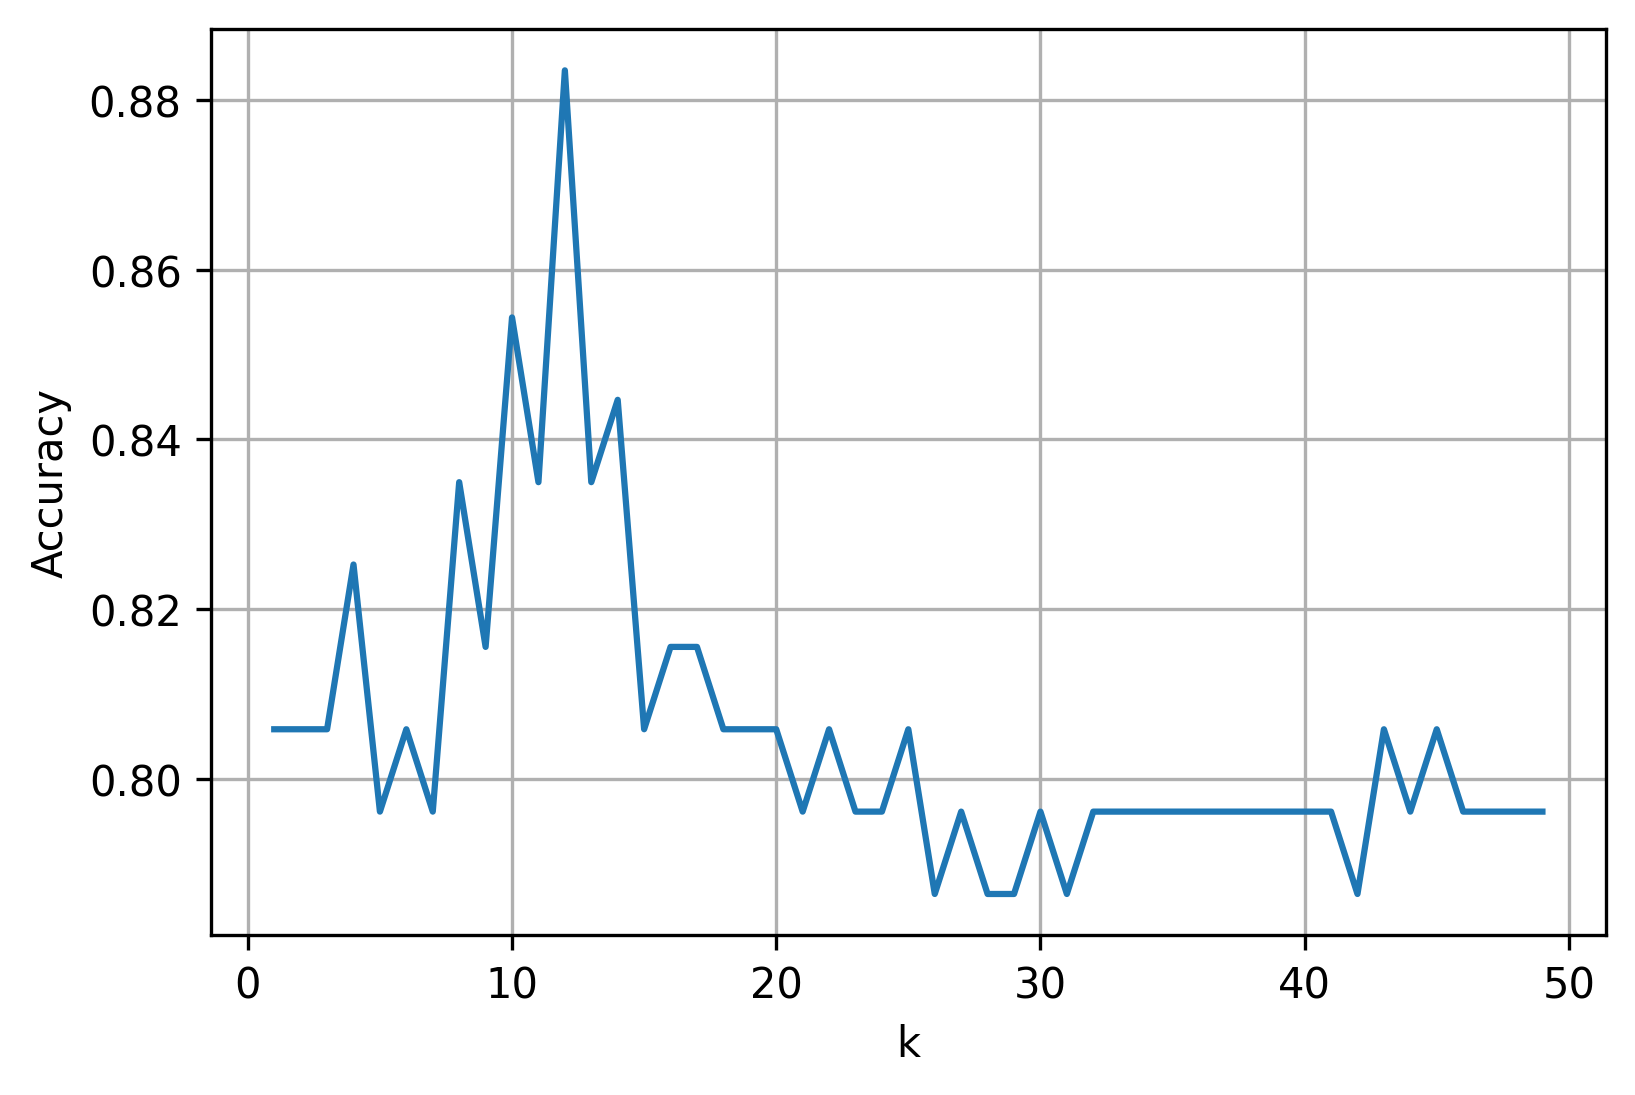
\includegraphics[width=.7\linewidth]{img/k_acc.png}
    \caption{Accuracy of the $k$-NN model, which uses the $\ell^2$ norm to do a weighted classification, for the number of nearest neighbours $k$.}
    \label{fig:k_acc}
\end{figure}

\begin{figure}[ht!]
    \centering
    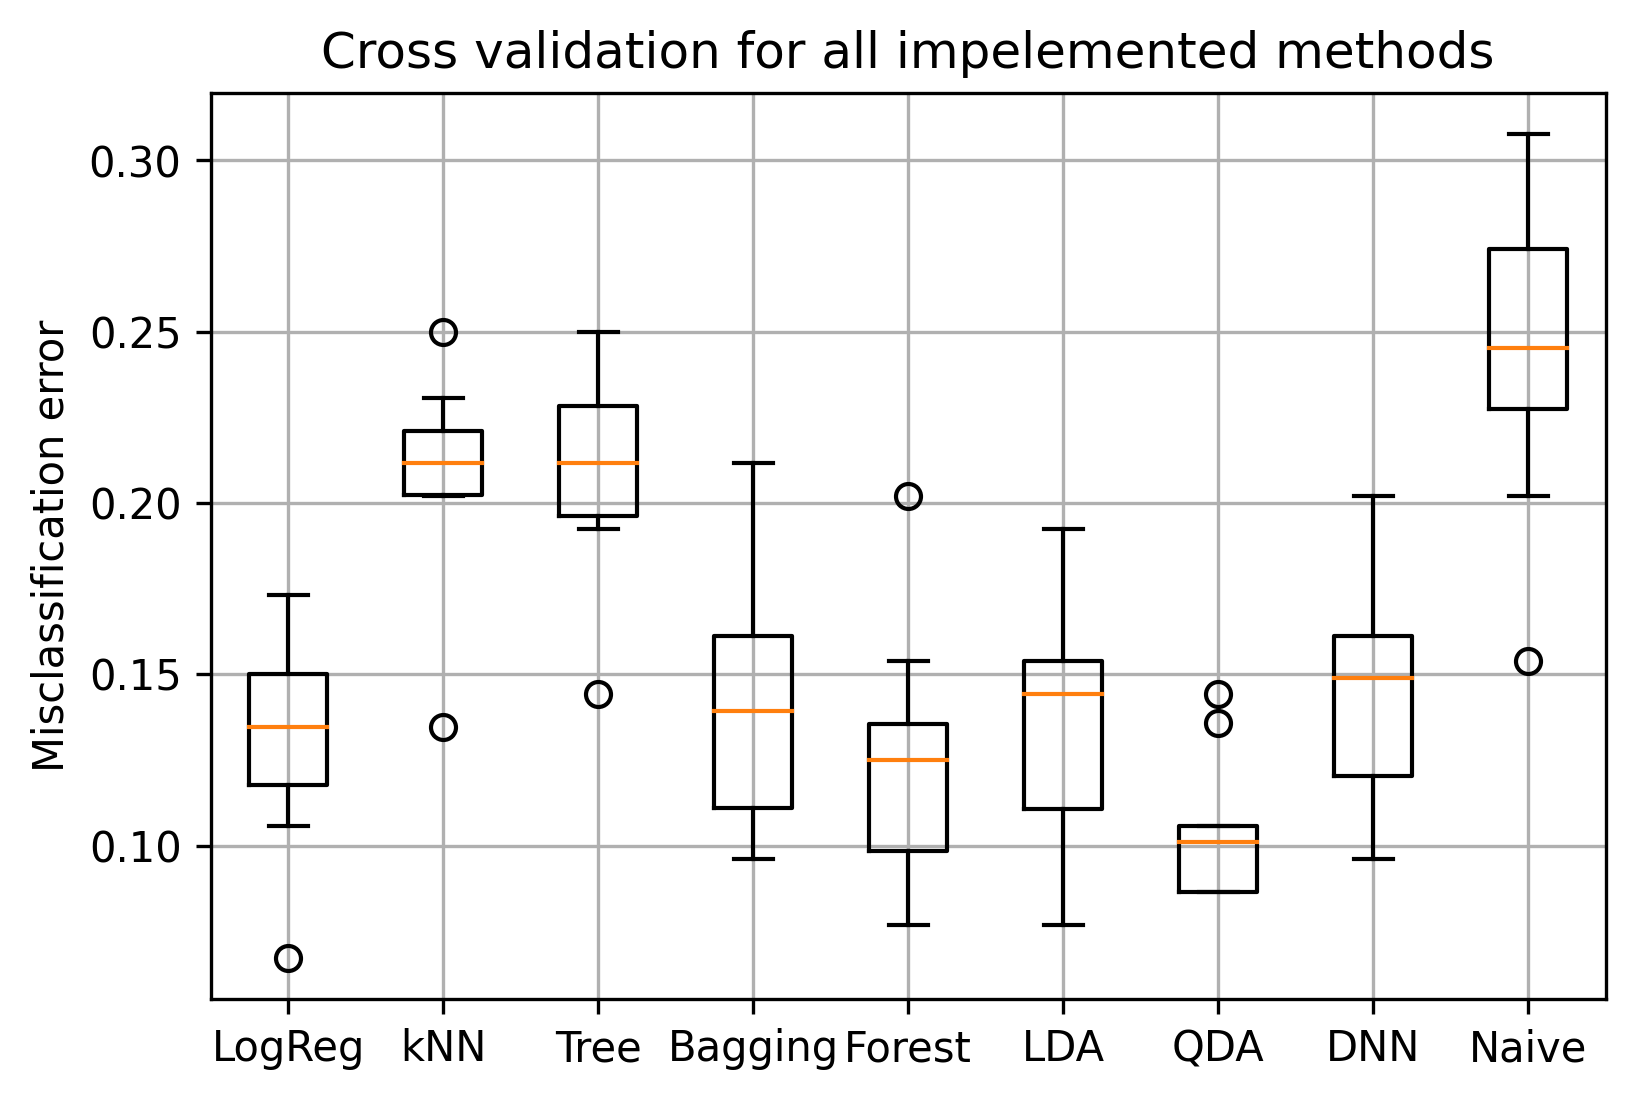
\includegraphics[width=.7\linewidth]{img/crossval.png}
    \caption{Box plot of performance of all optimized models.}
    \label{fig:cross}
\end{figure}

\newpage

\begin{landscape}
\begin{figure}[ht!]
    \centering
    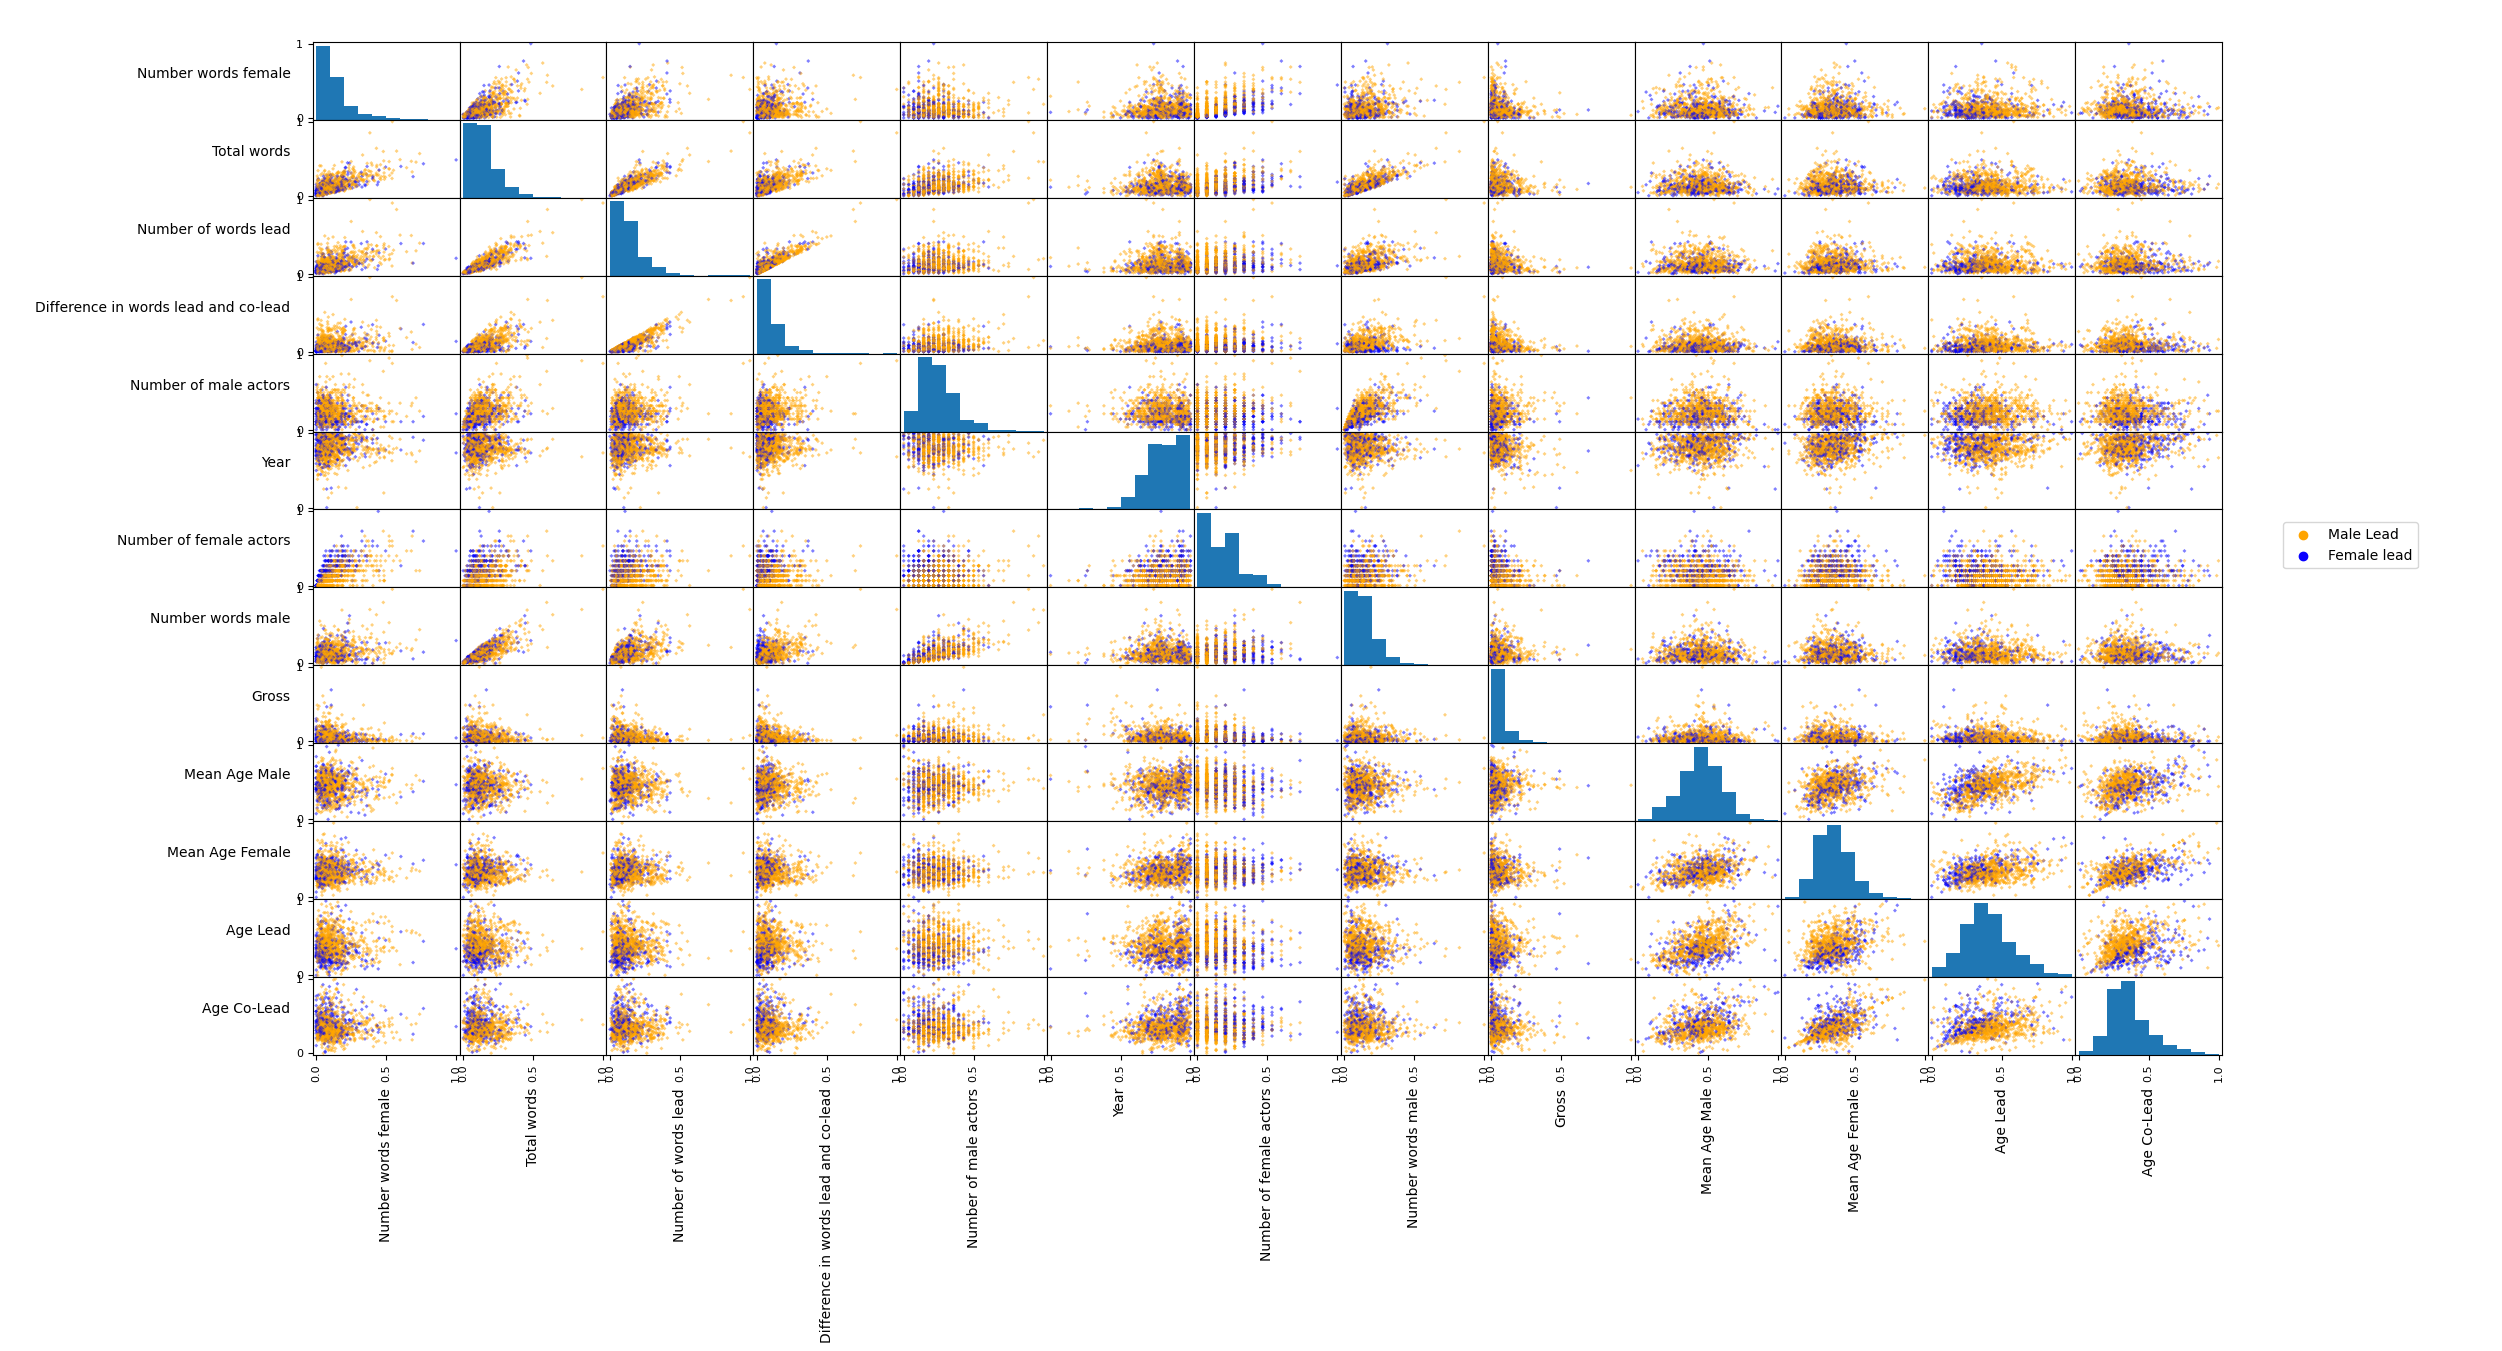
\includegraphics[width=240mm]{img/minmaxscale_hist_scatt.png}
    \caption{Histogram and scatter plot.}
    \label{fig:scatter}
\end{figure}
\end{landscape}

\textbf{Supplementary code for the reproduction of results}. A lot of the code is inspired by or taken from the exercise sheets of the Statistical Machine Learning course \cite{smlexercises}. These, in turn, use a lot of functions from external python libraries \cite{Covariance,bagtree,crossval,dectree,Gridser,kfold,Logreg,matplotlib,MinMax,Polyfit,randtree,Regul,scatter_mat,StandardScaler}.

\begin{minted}[linenos]{python}
''' Data analysis '''

import pandas as pd
import matplotlib.pyplot as plt
import seaborn as sns
import numpy as np
from sklearn.preprocessing import StandardScaler

training = pd.read_csv('data/train.csv')

features = ['Number words female','Total words','Number of words lead',
            'Difference in words lead and co-lead',
            'Number of male actors','Year','Number of female actors',
            'Number words male','Gross','Mean Age Male',
            'Mean Age Female','Age Lead','Age Co-Lead']

lead = [[sum(training.loc[:, "Number of female actors"]), 
        sum(training.loc[:, "Number of male actors"])]]
fm = pd.DataFrame(lead, columns=['Female', 'Male'])

firstyear = min(training.loc[:, 'Year'])
lastyear = max(training.loc[:, 'Year'])
''' try to compare the number of actors total per year with '''

lst = [x for x in range(firstyear, lastyear + 1, 1)]

numbermalactors = [];
numberfemalactors = [];
distro = [];
for year in range(firstyear, lastyear + 1, 1):
    thisyear = training[training.Year == year]
    if sum(thisyear.loc[:, 'Number of female actors'] + 
        thisyear.loc[:, 'Number of male actors']) > 0:
        distro.append(sum(thisyear.loc[:, 'Number of female actors']) /
            (sum(thisyear.loc[:, 'Number of female actors'] + 
            thisyear.loc[:, 'Number of male actors'])))
    else:
        distro.append(0)

Movies_with_more_male_speaking = training[training.loc[:, 'Number words male'] > 
                                training.loc[:, 'Number words female']]
Movies_with_more_female_speaking = training[training.loc[:, 'Number words male'] < 
                                training.loc[:, 'Number words female']]

mean_male_gross = np.mean(Movies_with_more_male_speaking.Gross)
mean_female_gross = np.mean(Movies_with_more_female_speaking.Gross)

distrosort1 = []
distrosort2 = []
for x in range(len(distro)):
    if distro[x] > 0:
        distrosort1.append(lst[x])
        distrosort2.append(distro[x])

a, b = np.polyfit(distrosort1, distrosort2, 1)

plt.figure(99)
plt.subplot(2, 2, 1)
sns.barplot(fm)
plt.title('Total number of female and male actors ' + 
            str(firstyear) + '-' + str(lastyear))
plt.subplot(2, 2, 2)
plt.grid()
for x in range(len(distro)):
    if distro[x] > 0:
        plt.scatter(lst[x], distro[x], color='blue')

string1 = f"{mean_male_gross:.{2}f}"
string2 = f"{mean_female_gross:.{2}f}"
plt.plot(lst, np.array(lst) * a + b, color='red')
plt.title('Percentage of female actors year by year')
plt.legend()
plt.subplot(2, 2, 3)
# plt.grid()
plt.scatter(Movies_with_more_male_speaking.loc[:, 'Year'], 
            Movies_with_more_male_speaking.Gross, color='orange',
            label='Male Lead')
plt.scatter(Movies_with_more_female_speaking.loc[:, 'Year'], 
            Movies_with_more_female_speaking.Gross, color='blue',
            label='Female lead')
plt.xlabel('Year')
plt.ylabel('Gross')
plt.legend()
plt.title('Gross - Dominant speaker')
plt.show()


scaler = StandardScaler()
Y = training.Lead
Y = Y.replace(to_replace=['Male', 'Female'], value=['orange', 'blue'])

training_x = training.drop(columns='Lead')
training_scaled = StandardScaler().fit_transform(training_x.values)
new = pd.DataFrame(training_scaled, index=training_x.index, 
                    columns=training_x.columns)

axes = pd.plotting.scatter_matrix(new, c=Y, s=4, marker='D')
for ax in axes.flatten():
    ax.xaxis.label.set_rotation(90)
    ax.yaxis.label.set_rotation(0)
    ax.yaxis.label.set_ha('right')

plt.show()

'''
inspired by:
https://stackoverflow.com/questions/58623528/pandas-scatter-matrix-
labels-vertical-x-and-horizontal-y-without-being-cut
'''
\end{minted}

\begin{minted}[linenos]{python}
'''Logistic regression '''

import sklearn.linear_model as skl_lm
import pandas as pd
import matplotlib.pyplot as plt
from sklearn.model_selection import cross_val_score
from sklearn.model_selection import GridSearchCV
import itertools
import numpy as np
from sklearn.preprocessing import StandardScaler


np.random.seed(1)

training = pd.read_csv('data/train.csv')
features = ['Number words female','Total words','Number of words lead',
            'Difference in words lead and co-lead',
            'Number of male actors','Year','Number of female actors',
            'Number words male','Gross','Mean Age Male',
            'Mean Age Female','Age Lead','Age Co-Lead']


trainI = np.random.choice(training.shape[0], size=1039, 
            replace=False)
trainIndex = training.index.isin(trainI)
scaler = StandardScaler()
training = training.replace(to_replace=['Male', 'Female'], 
            value=[0, 1])

train = training.iloc[trainIndex]
test = training.iloc[~trainIndex]


Y_train = train['Lead']
X_train = train[features]

training_scaled = StandardScaler().fit_transform(X_train.values)
X_train = pd.DataFrame(training_scaled, 
            index=X_train.index, columns=X_train.columns)


'''Select solver for testing all feature combination'''

test_solver = 'lbfgs' #'saga' 'sag' 'newton-cg' 'liblinear'


'''Test all combinations of features with selected 
    solver with standard hyperparameters'''
    
result = 0
best_features_cv = 0
for L in range(1, len(features) + 1, 1):
    for subset in itertools.combinations(features, L):
        model = skl_lm.LogisticRegression(solver=test_solver)
        X_train_iter = X_train[list(subset)]
        #X_test_iter = X_test[list(subset)]
        model.fit(X_train_iter, Y_train)
        mean_cross = np.mean(cross_val_score(model, X_train_iter, Y_train, cv=10))
        if mean_cross > result:
            result = mean_cross
            best_features_cv = list(subset)

print('Best result combinations: ' + str(result) + ' ' + str(best_features_cv))

'''
Inspiration:
https://stackoverflow.com/questions/464864/how-to-
get-all-possible-combinations-of-a-list-s-elements
https://bobbyhadz.com/blog/python-find-max-value-in-list-of-lists
'''


print(best_features_cv)

'''Tune with the best solver and features from above'''

hyperparameters = {'penalty':['l1','l2'],'C': np.logspace(-3,3,7),
                    'solver' : ['lbfgs']}

logr = skl_lm.LogisticRegression()
clf = GridSearchCV(logr,                   # model
                   param_grid = hyperparameters,
                   scoring='accuracy',        # metric
                   cv=10)                     # folds

'''
Inspiration: 
https://towardsdatascience.com/tuning-the-hyperparameters-of-
your-machine-learning-model-using-gridsearchcv-7fc2bb76ff27
'''

X_train = X_train[best_features_cv]
clf.fit(X_train,Y_train)

print("Tuned Hyperparameters :", clf.best_params_)
print("Accuracy :", clf.best_score_)


\end{minted}

\begin{minted}[linenos]{python}
'''kNN'''

import sklearn.neighbors as skl_nb
import sklearn.model_selection as skl_ms
import pandas as pd
import matplotlib.pyplot as plt
import numpy as np
from sklearn.preprocessing import StandardScaler
import itertools


train = pd.read_csv(url)
np.random.seed(1)

features = ['Number words female', 'Total words', 'Number of words lead', 'Difference in words lead and co-lead',
            'Number of male actors', 'Year', 'Number of female actors', 'Number words male', 'Gross', 'Mean Age Male',
            'Mean Age Female', 'Age Lead', 'Age Co-Lead']
X = train[features]
Y = train['Lead']

n_fold = 10  # Number of cross-validations
cv = skl_ms.KFold(n_splits=n_fold, random_state=2, shuffle=True)
K = np.arange(1, 50)
# Initialize array to save precision for each k for the various combinations of inputs
precision = np.zeros(
    (378, len(K)))  # 378 = sum_{i=10 to 13} BinomialCoef(13,i), number of different combinations to pick from
combinations = []
i = 0
for L in range(10, len(features) + 1, 1):  # Loop over features
    for subset in itertools.combinations(features, L):
        print(i, subset)
        for train_index, val_index in cv.split(X):
            X_train, X_val = X.iloc[train_index][list(subset)], X.iloc[val_index][list(subset)]
            y_train, y_val = Y.iloc[train_index], Y.iloc[val_index]
            for j, k in enumerate(K):
                scaler = StandardScaler().fit(X_train)
                # knn=skl_nb.KNeighborsClassifier(n_neighbors=k,p=3,metric='minkowski') #l^3 unweighted
                knn = skl_nb.KNeighborsClassifier(n_neighbors=k, metric='l2', weights='distance')  # l^2 weighted
                # knn=skl_nb.KNeighborsClassifier(n_neighbors=k,metric='l2') #l^2 unweighted
                # knn=skl_nb.KNeighborsClassifier(n_neighbors=k,metric='l1') #l^1 unweighted
                # knn=skl_nb.KNeighborsClassifier(n_neighbors=k,metric='l1', weights='distance') #l^1 weighted
                knn.fit(scaler.transform(X_train), y_train)
                prediction = knn.predict(scaler.transform(X_val))
                precision[i, j] = np.mean(prediction == y_val)
        combinations.append(subset)
        i += 1

best_index = list(np.unravel_index(np.argmax(precision), precision.shape))
print(best_index)
knn_features = list(combinations[best_index[0]])
print("Maximum CV accuracy is " + str(np.amax(precision)))
print("Best set of features is " + str(knn_features) + ", with k=" + str(best_index[1] + 1))
print(precision)

knn = skl_nb.KNeighborsClassifier(n_neighbors=k, metric='l2', weights='distance')  # l^2 weighted
knn_features = ['Number words female', 'Total words', 'Difference in words lead and co-lead', 'Number of male actors',
                'Year', 'Number of female actors', 'Number words male', 'Mean Age Male', 'Age Lead', 'Age Co-Lead']
k = 14

plt.grid()
plt.plot(K, precision[best_index[0], :])
plt.xlabel("k")
plt.ylabel("Accuracy")

X_train = train[knn_features]
y_train = train["Lead"]
scaler = StandardScaler().fit(X_train)
# knn=skl_nb.KNeighborsClassifier(n_neighbors=K[best_index[1]+1])
# knn.fit(scaler.transform(X_train),y_train)

knn = skl_nb.KNeighborsClassifier(n_neighbors=6)
knn.fit(scaler.transform(X_train), y_train)
models.append(knn)
print("Accuracy over the whole training set is " + str(np.mean(knn.predict(scaler.transform(X_train)) == y_train)))
\end{minted}

\begin{minted}[linenos]{python}
'''LDA/QDA'''

import sklearn.discriminant_analysis as skl_da
import pandas as pd
import matplotlib.pyplot as plt
import numpy as np

url = 'https://raw.githubusercontent.com/Falk0/sml_data/main/train.csv'
training = pd.read_csv(url)

test_url = 'https://raw.githubusercontent.com/Falk0/sml_data/main/test.csv'
test = pd.read_csv(test_url)

Train = pd.read_csv(url)
Test = pd.read_csv(test_url)
Train.head()

# Initiate training parameters
Parameters = ['Number words female', 'Total words', 'Number of words lead', \
              'Difference in words lead and co-lead', 'Number of male actors', \
              'Year', 'Number of female actors', 'Number words male', \
              'Gross', 'Mean Age Male', 'Mean Age Female', \
              'Age Lead', 'Age Co-Lead']

# Training
X_train = Train[Parameters]
Y_train = Train['Lead']

# LDA initializing and testing
from sklearn.discriminant_analysis import LinearDiscriminantAnalysis

# Creating model and use it to fit the training data
model = LinearDiscriminantAnalysis()
model.fit(X_train, Y_train)

# Calculating the probabilities and converting them into predictions
probabilities = model.predict_proba(X_train)
prediction = np.where(probabilities[:, 0] >= 0.5, 'Female', 'Male')

# Compare to true value
error = np.mean(prediction != Y_train)
print(pd.crosstab(prediction, Y_train))

# QDA initializing and testing
from sklearn.discriminant_analysis import QuadraticDiscriminantAnalysis

# Creating model and use it to fit the training data
model = QuadraticDiscriminantAnalysis()
model.fit(X_train, Y_train)

# Calculating the probabilities and converting them into predictions
predict_prob = model.predict_proba(X_train)
prediction = np.where(predict_prob[:, 0] >= 0.5, 'Female', 'Male')

# Compare to true value
error = np.mean(prediction != Y_train)
print(pd.crosstab(prediction, Y_train))

# Hyperparameter for LDA
import sklearn.model_selection as skl_ms
from sklearn import model_selection


# Function for varying the regularization parameter
def hyperparameter_testing(X, Y, sol, shr):
    # Initializing
    n_splits = 10
    misclassification = np.zeros(n_splits)

    # Model
    model = skl_da.LinearDiscriminantAnalysis(solver=sol, shrinkage=shr)

    # Evaluation of method
    cv = model_selection.KFold(n_splits=10, random_state=1, shuffle=True)

    # Model Testing
    model.fit(X, Y)
    prediction = model.predict(X)
    misclassification = np.mean(prediction != Y)

    return misclassification


# Shrinkage in range [0,1] and all solvers for LDA
Shrink = np.linspace(0.01, 0.99, 100)
Solver = ['svd', 'lsqr', 'eigen']

LDA = np.zeros([len(Shrink), len(Solver)])

# Defining input and output
X = Train.drop(columns=['Lead'])
Y = Train['Lead']

for i in range(len(Solver)):

    if Solver[i] == 'svd':
        Shrink = [None] * 100

    for j in range(len(Shrink)):
        Miss = hyperparameter_testing(X, Y, Solver[i], Shrink[j])
        LDA[j, i] = np.mean(Miss)

    Shrink = np.linspace(0.01, 0.99, 100)
    print(f'For {Solver[i]} we find that the minimal error to be: {min(LDA[:, i])}')
    if Solver[i] == 'svd':
        None
    else:
        location = np.where(LDA[:, i] == np.min(LDA[:, i]))
        print(f'This value is found with a shrinkage of {location[0]}')

lda = model = skl_da.LinearDiscriminantAnalysis(solver='svd')
models.append(lda)

# %% Regularization parameter for QDA

# Creating list
reg_testing = []


def hyperparameter_testing(X, Y, reg_param):
    # Initializing
    n_splits = 10
    misclassification = np.zeros(n_splits)

    # Model
    model = QuadraticDiscriminantAnalysis(reg_param=reg_param)

    # Evaluation of method
    cv = model_selection.KFold(n_splits=n_splits, random_state=1, shuffle=True)

    # Model Testing
    model.fit(X, Y)
    prediction = model.predict(X)
    misclassification = np.mean(prediction != Y)

    return misclassification


# parameter linspace
regularization = np.linspace(0.01, 0.99, 100)

# Defining input and output
X = Train.drop(columns=['Lead'])
Y = Train['Lead']

for i in regularization:
    test = hyperparameter_testing(X, Y, i)
    reg_testing.append(np.mean(test))

# Finding best parameter setting
index = reg_testing.index(min(reg_testing))
best = regularization[index]

plt.figure()
plt.plot(regularization, reg_testing)
plt.xlabel('Regularization parameter')
plt.ylabel('Error')
plt.show()

print(f'We find the best regularization parameter to be: {best}')


# Feature accuracy

def input_testing(X, Y, reg_param):
    # Initializing
    n_splits = 10
    n_fold = 10
    misclassification = np.zeros(n_splits)

    # Model (here we do both for efficiency)
    models_test = []
    models_test.append(skl_da.LinearDiscriminantAnalysis())
    models_test.append(skl_da.QuadraticDiscriminantAnalysis(reg_param=reg_param))

    misclassification = np.zeros((n_fold, len(models_test)))

    # Evaluation of method
    cv = model_selection.KFold(n_splits=n_splits, random_state=1, shuffle=True)

    # Model Testing
    for i, (train_index, val_index) in enumerate(cv.split(X)):
        X_train, X_val = X.iloc[train_index], X.iloc[val_index]
        Y_train, Y_val = Y.iloc[train_index], Y.iloc[val_index]

        # Appending both models
        for j in range(np.shape(models_test)[0]):
            # Testing both models
            model = models_test[j]
            model.fit(X_train, Y_train)
            prediction = model.predict(X_val)
            # Accuracy based on each model
            misclassification[i, j] = np.mean(prediction != Y_val)

    return misclassification


# New lists for each model
LDA_accuracy = []
QDA_accuracy = []

# First a reference point without any missing data
X = Train.drop(columns=['Lead'])
Y = Train['Lead']
Accuracy = input_testing(X, Y, 0.25)
LDA_accuracy.append(Accuracy[:, 0])
QDA_accuracy.append(Accuracy[:, 1])

# Here we use dataset with 1 missing parameter at the time
for i in range(len(Parameters)):
    # Define data for the variable
    X = Train.drop(columns=[Parameters[i], 'Lead'])
    Y = Train['Lead']

    Accuracy = input_testing(X, Y, 0.25)

    LDA_accuracy.append(Accuracy[:, 0])
    QDA_accuracy.append(Accuracy[:, 1])

# Plotting
plt.figure()
plt.boxplot(LDA_accuracy)
plt.show()

plt.figure()
plt.boxplot(QDA_accuracy)
plt.show()

# Accuracies
for i in range(14):
    print(np.mean(LDA_accuracy[i]))

for i in range(14):
    print(np.mean(QDA_accuracy[i]))

model = skl_da.QuadraticDiscriminantAnalysis(reg_param=0.495050505050505)
models.append(model)

\end{minted}

\begin{minted}[linenos]{python}
'''Tree/Bagging/Forest'''
import pandas as pd
import numpy as np
import time
import sys
from sklearn.tree import DecisionTreeClassifier
from sklearn.ensemble import RandomForestClassifier, BaggingClassifier
from sklearn.model_selection import GridSearchCV, cross_validate
import itertools


def main(argv):
    train_df = pd.read_csv(argv[0]).replace(to_replace=['Male', 'Female'], value=[0, 1])

    features = ['Number words female', 'Total words', 'Number of words lead', 'Difference in words lead and co-lead',
                'Number of male actors', 'Year', 'Number of female actors', 'Number words male', 'Gross',
                'Mean Age Male',
                'Mean Age Female', 'Age Lead', 'Age Co-Lead']
    x_train = train_df[features]
    y_train = train_df['Lead']

    # DecisionTree
    # Feature Selection
    result = []
    for L in range(1, len(features) + 1, 1):
        print(L)
        for subset in itertools.combinations(features, L):
            model = DecisionTreeClassifier()
            x_train = train_df[list(subset)]
            model.fit(x_train, y_train)
            result.append([np.mean(cross_validate(model, x_train, y_train, cv=10)['test_score']), subset])
    print('Best result combinations: ' + str(max(result, key=lambda sublist: sublist[0])))
    # Hyperparametertuning
    d_param_dist = {'max_depth': [*range(1, 10), None],
                    'min_samples_split': [*range(2, 10)],
                    'min_samples_leaf': [*range(1, 10)],
                    'max_features': ['sqrt', 'log2'],
                    'splitter': ['best', 'random'],
                    'criterion': ['gini', 'entropy', 'log_loss']}
    d_best_features = ['Number words female', 'Number of words lead', 'Difference in words lead and co-lead',
                       'Number of male actors', 'Number of female actors', 'Number words male', 'Age Lead']
    d_x_train = train_df[d_best_features]
    d_tree = DecisionTreeClassifier()
    d_gridsearch = GridSearchCV(d_tree, param_grid=d_param_dist, scoring='accuracy', cv=10)
    d_gridsearch.fit(d_x_train, y_train)
    print(f'decision tree, best params: {d_gridsearch.best_params_}')
    print(f'decision tree, best accuracy: {d_gridsearch.best_score_}')

    # RandomForest
    # Feature Selection
    result = []
    for L in range(1, len(features) + 1, 1):
        print(L)
        for subset in itertools.combinations(features, L):
            model = RandomForestClassifier()
            x_train = train_df[list(subset)]
            model.fit(x_train, y_train)
            result.append([np.mean(cross_validate(model, x_train, y_train, cv=10)['test_score']), subset])
    print('Best result combinations: ' + str(max(result, key=lambda sublist: sublist[0])))
    r_best_features = ['Number words female', 'Number of words lead', 'Difference in words lead and co-lead', 'Number of male actors', 'Number of female actors', 'Number words male', 'Age Co-Lead']
    r_x_train = train_df[r_best_features]
    # Hyperparametertuning
    r_param_dist = {'n_estimators': [*range(10)],
                    'max_depth': [*range(1, 10), None],
                    'min_samples_split': [*range(2, 10)],
                    'min_samples_leaf': [*range(1, 10)],
                    'max_features': ['sqrt', 'log2', None],
                    'criterion': ['gini', 'entropy', 'log_loss']}
    r_tree = RandomForestClassifier()
    r_gridsearch = GridSearchCV(r_tree, param_grid=r_param_dist, scoring='accuracy', cv=10)
    r_gridsearch.fit(r_x_train, y_train)
    print(f'random forest, best params: {r_gridsearch.best_params_}')
    print(f'random forest, tree, best accuracy: {r_gridsearch.best_score_}')

    # Bagging
    # Feature Selection
    result = []
    for L in range(1, len(features) + 1, 1):
        print(L)
        for subset in itertools.combinations(features, L):
            model = BaggingClassifier()
            x_train = train_df[list(subset)]
            model.fit(x_train, y_train)
            result.append([np.mean(cross_validate(model, x_train, y_train, cv=10)['test_score']), subset])
    print('Best result combinations: ' + str(max(result, key=lambda sublist: sublist[0])))
    b_best_features = ['Number words female', 'Number of words lead', 'Difference in words lead and co-lead',
                       'Number of male actors', 'Number of female actors', 'Number words male', 'Mean Age Female']
    # Final Models

    d_tree_final = DecisionTreeClassifier(max_depth=6, min_samples_split=3, min_samples_leaf=5, max_features='log2',
                                          splitter='best', criterion='gini')
    d_tree_final.fit(d_x_train, y_train)
    r_tree_final = RandomForestClassifier(n_estimators=8, max_depth=9, min_samples_split=6, min_samples_leaf=4,
                                          max_features=None, criterion='entropy')
    r_tree_final.fit(r_x_train, y_train)
    b_tree_final = BaggingClassifier(n_estimators=11, max_samples=8, bootstrap='True', max_features=6,
                                     bootstrap_features='False', oob_score='True')
    b_tree_final.fit(b_x_train, y_train)

    # models.append(d_tree_final, r_tree_final, b_tree_final)


if __name__ == '__main__':
    tic = time.perf_counter()
    main(sys.argv[1:])
    toc = time.perf_counter()
    print(f"Finished in {toc - tic:0.4f} seconds")


\end{minted}
 


\begin{minted}[linenos]{python}
'''Deep learning'''


import tensorflow as tf
training = pd.read_csv(url)
training = training.replace(to_replace=['Male', 'Female'], value=[0, 1])


'''M = 200
idx = training.index.values[training['Lead'] == 0][:M]
training = training.drop(idx)'''

trainI = np.random.choice(training.shape[0], size=int(0.8*len(training)), replace=False)
trainIndex = training.index.isin(trainI)

train = training.iloc[trainIndex]
test = training.iloc[~trainIndex]

features = ['Number words female','Total words','Number of words lead','Difference in words lead and co-lead',
            'Number of male actors','Year','Number of female actors','Number words male','Gross','Mean Age Male',
            'Mean Age Female','Age Lead','Age Co-Lead']

X_train = train[features]
Y_train = train['Lead']
X_test = test[features]
Y_test = test['Lead']


model = tf.keras.Sequential()
model.add(tf.keras.layers.Dense(128, input_dim=13, activation='relu')) 
model.add(tf.keras.layers.Dense(64, activation='relu'))
model.add(tf.keras.layers.Dense(32, activation='relu')) 
model.add(tf.keras.layers.Dense(1, activation='sigmoid'))

model.compile(
  loss=tf.keras.losses.binary_crossentropy,
  optimizer=tf.keras.optimizers.Adam(lr=0.001),
  metrics=[
      tf.keras.metrics.BinaryAccuracy(name='accuracy'),
      tf.keras.metrics.Precision(name='precision'),
      tf.keras.metrics.Recall(name='recall')
    ]
)

history = model.fit(X_test, Y_test, epochs=100)

dnn = model

\end{minted}

\begin{minted}[linenos]{python}
'''Cross validation, test all models, and predictions with the best model'''


np.random.seed(1)
n_fold=10
misclassification=np.zeros((10,9))
cv=skl_ms.KFold(n_splits=n_fold,random_state=1,shuffle=True)
for i, (train_index, val_index) in enumerate(cv.split(training)): 
  y_train, y_val = Y_train.iloc[train_index], Y_train.iloc[val_index]
  x_train, x_val = training.iloc[train_index], training.iloc[val_index]

  scaler = StandardScaler()
  scaler.fit(x_train)
  scaled_x_train_tr = scaler.transform(x_train.values)
  scaled_x_train = pd.DataFrame(scaled_x_train_tr,  index=x_train.index, columns=x_train.columns)
  scaled_x_val_tr = scaler.transform(x_val.values)
  scaled_x_val = pd.DataFrame(scaled_x_val_tr,  index=x_val.index, columns=x_val.columns)


  for m in range(np.shape(models)[0]):
    model=models[m]
    if model == dnn:
        prediction = model.predict(x_val)
        prediction_classes = [1 if prob > 0.5 else 0 for prob in np.ravel(prediction)]
        prediction = prediction_classes
    elif model == logreg:
        model.fit(scaled_x_train[logreg_features],y_train)
        prediction = model.predict(scaled_x_val[logreg_features])

    elif model == knn:
        model.fit(scaled_x_train[knn_features],y_train)
        prediction = model.predict(scaled_x_val[knn_features])

    elif model == lda:
        X_train = x_train[lda_features]
        model.fit(X_train,y_train)
        prediction = model.predict(x_val[lda_features])

    elif model == qda:
        X_train = x_train[qda_features]
        model.fit(X_train,y_train)
        prediction = model.predict(x_val[qda_features])

    elif model == d_tree_final:
        X_train = x_train[d_best_features]
        model.fit(X_train,y_train)
        prediction = model.predict(x_val[d_best_features])

    elif model == b_tree_final:
        X_train = x_train[b_best_features]
        model.fit(X_train,y_train)
        prediction = model.predict(x_val[b_best_features])

    elif model == r_tree_final:
        X_train = x_train[r_best_features]
        model.fit(X_train,y_train)
        prediction = model.predict(x_val[r_best_features])

    elif model == 'dummy':
        prediction = np.zeros(len(x_val))
    
    misclassification[i,m]=np.mean(prediction!=y_val)

plt.boxplot(misclassification)
plt.title("Cross validation for all impelemented methods")
plt.ylabel("Misclassification error")
plt.xticks(np.arange(9)+1,("LogReg","kNN","Tree", "Bagging", "Forest","LDA", "QDA", "DNN", "Naive"))
plt.grid()
plt.show()
print(models)

import csv
'final method'

training = pd.read_csv(url)
qda_features_final = ['Number words female','Total words','Number of words lead','Difference in words lead and co-lead',
                      'Number of male actors','Number of female actors','Number words male','Gross','Mean Age Male',
                      'Mean Age Female','Age Lead','Age Co-Lead']
training = training.replace(to_replace=['Male', 'Female'], value=[0, 1])
y_train = training['Lead']
x_train = training[qda_features_final]
test_url = 'https://raw.githubusercontent.com/Falk0/sml_data/main/test.csv'
x_test = pd.read_csv(test_url)
x_test = x_test[qda_features_final]

final = skl_da.QuadraticDiscriminantAnalysis(reg_param=0.495050505050505)

final.fit(x_train,y_train)

prediction_final = final.predict(x_test)

with open('final.csv', 'w') as f:
  writer = csv.writer(f)
  writer.writerow(prediction_final)

\end{minted}



\bibliographystyle{ieeetr}
\bibliography{ref}
\end{document}
